% nladoc.tex V2.0, 13 May 2010

\RequirePackage{fix-cm}
\documentclass[smallcondensed,final]{svjour3}     % onecolumn (ditto)

\usepackage{moreverb}

\usepackage[colorlinks,bookmarksopen,bookmarksnumbered,citecolor=red,urlcolor=red]{hyperref}
\usepackage{tikz}
\usetikzlibrary{shapes,arrows,trees,snakes} %,decorations.pathreplacing,fit}
% \usepackage{tkz-euclide}
\usepackage{pgfplots}
\usepgfplotslibrary{external} 
\tikzexternalize
\usepackage{caption,subcaption}
% \usetkzobj{all} 
\usepackage{amsmath,amsfonts,amssymb}
\usepackage{cite}

\definecolor{utorange}{RGB}{203,96,21}
\definecolor{utblack}{RGB}{99,102,106}
\definecolor{utbrown}{RGB}{110,98,89}
\definecolor{utsecbrown}{RGB}{217,200,158}
\definecolor{utsecgreen}{RGB}{208,222,187}
\definecolor{utsecblue}{RGB}{127,169,174}


\newcommand{\todo}[1]{\textcolor{red}{\bf #1}}
\newcommand{\gsnote}[1]{\textcolor{blue}{GS: #1}}
\newcommand{\bs}[1]{\ensuremath{\boldsymbol #1}}


\newcommand\BibTeX{{\rmfamily B\kern-.05em \textsc{i\kern-.025em b}\kern-.08em
T\kern-.1667em\lower.7ex\hbox{E}\kern-.125emX}}

%\def\volumeyear{2013}

\begin{document}

\titlerunning{Comparison of high-order geometric multigrid methods}

\title{Comparison of Geometric Multigrid Algorithms for High-order Finite Element Discretizations}

\author{Hari Sundar, Georg Stadler, Omar Ghattas and George Biros}

\institute{Institute for Computational Engineering \& Sciences, The
  University of Texas at Austin, Austin, TX}

%\corraddr{\texttt{hari@ices.utexas.edu}}
\maketitle

\begin{abstract}
We are interested in asymptotically
optimal---$\mathcal{O}(N)$---complexity solvers for approximating the
solution of elliptic partial differential equations (PDEs), where $N$
is the number of unknowns.  Multigrid is such a solver. In practice
however, multigrid performs best for low-order uniform discretizations
with smooth coefficients.
%
Our goal is to compare different geometric multigrid approaches for
solving systems arising from high order discretizations of
variable-coefficient elliptic partial differential equations on
arbitrary geometries. High order discretizations offer several
advantages over low-order discretizations. Besides the faster
convergence per unknown for sufficiently smooth problems, high order
discretizations can often make better use of modern hardware due to
their locality, resulting in improved efficiency of the calculations.
%  According to standard isoparametric polynomial
%approximation theory, by using a finite element basis of at least
%degree $p$, we can achieve very fast $\mathcal{O}(N^{-(p+1)})$
%convergence for sufficiently smooth problems while improving the
%locality and thus the CPU efficiency of the calculations.
\end{abstract}

\keywords{geometric multigrid, high-order finite elements, spectral method, $p$-multigrid}



\section{Introduction}

This paper presents a systematic comparison of geometric multigrid
algorithms for the solution of systems arising from high-order (we
target polynomial orders up to 16) discretizations of elliptic partial
differential equations. Our particular interest is to compare the
efficiency of different high-order multigrid methods for problems with
varying coefficients and complex geometry.
% High-order discretization
High-order spatial discretizations can have significant advantages
over low-order methods, especially when the solution is smooth and
high accuracy is desired. However, the sparsity of finite element (or
finite difference) operators decreases as the polynomial approximation
order increases, which makes the application of high-order operators
to vectors computationally significantly more expensive. This is also
true if matrix-free methods are used, i.e., system matrices are never
assembled, but their application on vectors is implemented through
elemental loops.  Besides the loss of sparsity, another challenge in
high-order discretizations is due to the fact that the discretization
matrices loose structural properties such as the M-matrix property,
which often allows to prove convergence of iterative solvers.

While we use moderate size model problems for the comparisons in this
paper, we also discuss our findings with regard to parallel
implementations on high performance computing platforms.  In
particular, we discuss matrix-free methods, i.e., methods that do not
require assembled finite element matrices. This is critical for
high-order methods since the number of nonzero entries in finite
element matrices increases rapidly as the polynomial order
increases. For instance, for a three-dimensional hexahedral mesh
finite element discretizations with polynomial degree $p$, dense
element matrices are of size $(p+1)^3\times (p+1)^3$. For $p=8$, for
instance, this amounts to more than half a million entries
contributing to the globally assembled finite element matrix.  For
tensorized nodal basis functions on hexahedral meshes, the application
of elemental matrices to vectors can be implemented efficiently by
exploiting the tensor structure of the basis functions, as is common
for spectral elements, e.g.,~\cite{DevilleFischerMund02}. We use
geometry-resolving, isoparametric quadrilateral and hexahedral finite
elements in our comparisons. While this work is partly driven by our
interest in scalable parallel simulations on nonconforming meshes
derived from adaptive octrees (e.g.,\cite{SundarBirosBursteddeEtAl12,
  SampathBiros10, BursteddeGhattasGurnisEtAl10}, for the comparisons
presented in this paper we restrict ourselves to conforming meshes,
for simplicity.

Moreover, we consider parallelization aspects relevant for
implementations on shared or distributed memory architectures. For
instance, the implementation of Gauss-Seidel smoothers can be
challenging in parallel~\cite{AdamsBrezinaHuEtAl03,
  BakerFalgoutKolevEtAl11}; we thus include a Chebyshev-accelerated
Jacobi smoother in our comparisons. This polynomial smoother is as
easy to implement in parallel as Jacobi smoothing, but often yields a
performance that is comparable to Gauss-Seidel smoothing.

% The naive assembly and application
%of these elemental matrices requires $\mathcal O(p^9)$ operatrions,
%but exploiting the tensor structure of the basis functions allows to
%reduce this to $\mathcal O(p^7)$ operations

Multigrid for high-order/spectral finite elements has been studied as
early as in the 1980s. In~~\cite{RonquistPatera87}, the authors
observe that point smoothers such as the simple Jacobi method result
in resolution-independent convergence rates for high-order elements on
simple one and two dimensional geometries. Initial theoretical
evidence for this behavior is given in~\cite{MadayMunoz88}, where
multigrid convergence is studied for one-dimensional spectral methods
and spectral element problems. This high-order geometric multigrid
requires the computation of high-order residuals and high-order
interpolation and prolongation. Thus, an efficient implementation
cannot assemble these operators, i.e., has to be matrix-free.  In this
paper, we compare different smoothers for such a high-order
$h$-multigrid method on two and three dimensional complex geometries
with varying coefficients.

An alternative to this high-order geometric multigrid, which is based
on a mesh hierarchy is $p$-multigrid, which coarsens the polynomial
degree while (at least, initially) keeping the mesh unchained, see,
e.g.,~\cite{HelenbrookMavriplisAtkins03}. Here, we compare the
performance and this $p$-multigrid approach with $h$-multigrid for
different smoothers and polynomial orders.

%Even though high-order discretizations can, in principle, benefit from
%modern hardware, the rapid loss of sparsity of the involved systems as
%the polynomial order increases represents a significant challenge.

A popular strategy for high-order discretizations for unstructured
meshes, for which the application of geometric multigrid is
challenging, is to assemble a low-order approximation of the
high-order system and use an algebraic multigrid method to invert the
low order (and thus much sparser) operator~\cite{Brown10, Kim07,
  DevilleMund90, Olson07,
  CanutoGervasioQuarteroni10}. In~\cite{HeysManteuffelMcCormickEtAl05},
this approach is compared with the direct application of algebraic
multigrid to the high-order operator. In our test problems, we compare
the performance of this low-order preconditioning approach to the
performance obtained with $h$-multigrid and $p$-multigrid.

This paper is organized as follows \ldots

%\gsnote{Unify notion of mesh/grid etc}\\
% \gsnote{Unify use of high-order vs.\ higher order}\\
%\gsnote{We use hexas, motivated from spectral methods. Main
%  advantage is tensorized basis functions (and, potential octree adaptivity)}\\
%\gsnote{high-order discretizations map better to current architectures}


%Although there are examples of using Algebraic Multigrid directly on
%operators resulting from high-order discretizations, limited work
%has been done on using geometric multigrid with high-order
%discretizations. To the best of our knowledge, no prior work on using
%geometric multigrid for solving systems arising from high-order
%discretizations on arbitrary geometries using highly adapted meshes.

%In this work, we develop
%geometric multigrid methods to support higher-order discretizations
%($1\le p\le 8$) and compare  against preconditioning using the
%co-located linear operator.

% We evaluate using variable-coefficient
%Poisson problems on $2D$ and $3D$ domains. We demonstrate that by
%using appropriate inter-grid transfer operators and smoothers,
%mesh-independent convergence is possible ($1\le p\le8$) for the {\em
%direct} approach. For the direct approach, best results are obtained
%using the symmetric successive over-relaxation (SSOR) smoother. We
%conclude with thoughts on the parallelization of the proposed
%approach.\\[2ex]


%\section{Meshing, High-order FEM}


%Our method is designed for meshes that are built from an unstructured
%hexahedral macro mesh, in which each macro element is adaptively
%refined as an octree. This forest-of-octrees approach enables us to
%generate meshes for complex geometries with arbitrary levels of local
%refinement. We use geometric multigrid (GMG) for each of the octrees
%and algebraic multigrid (AMG) as the coarse grid solver. We designed
%our GMG sweeps to entirely avoid collectives, thus minimizing
%communication cost. Recently \cite{SundarBirosBursteddeEtAl12}, we
%presented weak and strong scaling results for the 3D
%variable-coefficient Poisson problem using linear discretization that
%demonstrate high parallel scalability. Here we explore various
%approaches for extending our geometric multigrid solver to support
%higher-order discretizations.


\section{Approaches for high-order geometric multigrid}
\label{sec:approaches}
% talk about the 4 main approaches and prior work.

In this section, we summarize different approaches to geometric
multigrid for high-order finite element discretizations; for an
illustrative overview see Figure~\ref{fig:approaches}. These methods
can either be directly used as solvers, or as preconditioners within a
Krylov method.

\begin{figure}
		% illustration for p-multigrid
		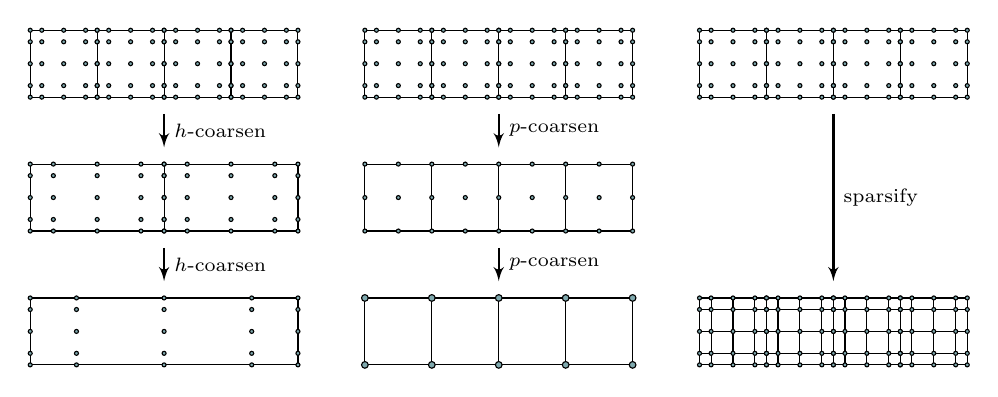
\begin{tikzpicture}[scale=0.85]
		% homg
		\draw (-5,4) grid +(4,1);
		\foreach \e in {-5,...,-2}
		\foreach \x in {0,0.1727,0.5,0.8273, 1.0} {
			\draw[fill=utsecblue] (\e+\x, 4) circle (0.03);
			\draw[fill=utsecblue] (\e+\x, 4.1727) circle (0.03);
			\draw[fill=utsecblue] (\e+\x, 4.5) circle (0.03);
			\draw[fill=utsecblue] (\e+\x, 4.8273) circle (0.03);
			\draw[fill=utsecblue] (\e+\x, 5) circle (0.03);
		}
		%\node at (5,4.5) {\small $p=4$};
		\draw[-latex',thick] (-3, 3.75) -- node[right] {{\scriptsize $h$-coarsen}} (-3, 3.25);
		\draw (-5,2) rectangle +(4,1);
		\draw (-3,2) -- (-3,3);
		\foreach \e in {-5,-3}
		\foreach \x in {0,0.1727,0.5,0.8273, 1.0} {
			\draw[fill=utsecblue] (\e+2*\x, 2) circle (0.03);
			\draw[fill=utsecblue] (\e+2*\x, 2.1727) circle (0.03);
			\draw[fill=utsecblue] (\e+2*\x, 2.5) circle (0.03);
			\draw[fill=utsecblue] (\e+2*\x, 2.8273) circle (0.03);
			\draw[fill=utsecblue] (\e+2*\x, 3) circle (0.03);
		}
		%\node at (5,2.5) {\small $p=2$};
	
		\draw[-latex',thick] (-3, 1.75) -- node[right] {{\scriptsize $h$-coarsen}} (-3, 1.25);
	
		\draw (-5,0) rectangle +(4,1);
		\foreach \x in {0,0.1727,0.5,0.8273, 1.0} {
			\draw[fill=utsecblue] (-5+4*\x, 0) circle (0.03);
			\draw[fill=utsecblue] (-5+4*\x, 0.1727) circle (0.03);
			\draw[fill=utsecblue] (-5+4*\x, 0.5) circle (0.03);
			\draw[fill=utsecblue] (-5+4*\x, 0.8273) circle (0.03);
			\draw[fill=utsecblue] (-5+4*\x, 1) circle (0.03);
		}
		
	%% p-multigrid
		\draw (0,4) grid +(4,1);
		\foreach \e in {0,...,3}
		\foreach \x in {0,0.1727,0.5,0.8273, 1.0} {
			\draw[fill=utsecblue] (\e+\x, 4) circle (0.03);
			\draw[fill=utsecblue] (\e+\x, 4.1727) circle (0.03);
			\draw[fill=utsecblue] (\e+\x, 4.5) circle (0.03);
			\draw[fill=utsecblue] (\e+\x, 4.8273) circle (0.03);
			\draw[fill=utsecblue] (\e+\x, 5) circle (0.03);
		}
		%\node at (5,4.5) {\small $p=4$};
	
		\draw[-latex',thick] (2, 3.75) -- node[right] {{\scriptsize $p$-coarsen}} (2, 3.25);
	
		\draw (0,2) grid +(4,1);
		\foreach \x in {0,0.5,...,4} {
			\draw[fill=utsecblue] (\x, 2) circle (0.03);
			\draw[fill=utsecblue] (\x, 2.5) circle (0.03);
			\draw[fill=utsecblue] (\x, 3) circle (0.03);
		}
		%\node at (5,2.5) {\small $p=2$};
	
		\draw[-latex',thick] (2, 1.75) -- node[right] {{\scriptsize $p$-coarsen}} (2, 1.25);
	
		\draw (0,0) grid +(4,1);
		\foreach \x in {0,1,2,3,4} {
			\draw[fill=utsecblue] (\x, 0) circle (0.05);
			\draw[fill=utsecblue] (\x, 1) circle (0.05);
		}
		%\node at (5,0.5) {\small $p=1$};
		
		%% collocated
			\draw (5,4) grid +(4,1);
			\foreach \e in {5,...,8}
			\foreach \x in {0,0.1727,0.5,0.8273, 1.0} {
				\draw[fill=utsecblue] (\e+\x, 4) circle (0.03);
				\draw[fill=utsecblue] (\e+\x, 4.1727) circle (0.03);
				\draw[fill=utsecblue] (\e+\x, 4.5) circle (0.03);
				\draw[fill=utsecblue] (\e+\x, 4.8273) circle (0.03);
				\draw[fill=utsecblue] (\e+\x, 5) circle (0.03);
			}
			%\node at (2, 1.8) {\tiny $p=4$};
	
			\draw[-latex',thick] (7, 3.75) -- node[right] {{\scriptsize sparsify}} (7, 1.25);
	
			\draw[step=0.5] (4.99,0) grid +(4.01,1);
			\draw (5,0.1727) -- (9,0.1727);
			\draw (5,0.8273) -- (9,0.8273);
			\foreach \e in {5,...,8} {
				\draw (\e+0.1727,0) -- (\e+0.1727,1);
				\draw (\e+0.8273,0) -- (\e+0.8273,1);
				\foreach \x in {0,0.1727,0.5,0.8273, 1.0} {
					\draw[fill=utsecblue] (\e+\x, 0) circle (0.03);
					\draw[fill=utsecblue] (\e+\x, 0.1727) circle (0.03);
					\draw[fill=utsecblue] (\e+\x, 0.5) circle (0.03);
					\draw[fill=utsecblue] (\e+\x, 0.8273) circle (0.03);
					\draw[fill=utsecblue] (\e+\x, 1) circle (0.03);
				}
			}
			% \node at (2, -0.2) {\tiny $p=1$ collocated with $p=4$};
		\end{tikzpicture}
		\caption{\label{fig:approaches} Different approaches
                  for high-order multigrid: high-order $h$-multigrid
                  (left), $p$-multigrid (middle) and low-order
                  preconditioned multigrid.}
\end{figure}

\subsection{$h$-multigrid}\label{subsec:h}
A direct approach to high-order multigrid is to use high-order
restriction and prolongation operators, and use the high-order
discretization of the operator for the residual computation on each
multigrid level.  A potential difficulty in this approach is that it
requires smoothers for matrices arising from high-order
discretization, which usually have less favorable properties compared
to their low order counterparts; For instance, high-order
discretizations of scalar elliptic operators are usually not
M-matrices, which is a useful property to prove the convergence of
smoothers such as Jacobi of Gauss-Seidel.  Due to the decreased
sparsity of high-order discretized systems, the efficient computation
of the residual can be a challenge. As a remedy, one can use
matrix-free methods which do not require to assemble system matrices
but rely on element-local computations. The performance of these
element-local computations can often be speed up using tensorized
finite element basis functions as common in spectral element methods;
see e.g.~\cite{DevilleFischerMund02}.


\subsection{$p$-multigrid}\label{subsec:p}
In the $p$-multigrid approach to high-order multigrid, one (initially)
does not coarsen the mesh geometrically, but coarsens the system by
reducing the polynomial order. Starting from an order-$p$ polynomial
basis (for simplicity, we assume here that $p$ is a power of 2), the
coarser grids correspond to polynomials of order $p/2, p/4,\ldots,1$,
followed by geometric coarsening of the $p=1$ grid (i.e., the usual
low order geometric multigrid). Decreasing the polynomial order is an
element-local operation and is particularly simple for discretizations
with nonconforming meshes. \gsnote{Is that actually true?}. As for
high-order $h$-multigrid, devising smoothers is a challenge for
$p$-multigrid.  Moreover, one often finds dependence of the
convergence factor on the order of the polynomial basis. \gsnote{We
  need a citation here.}

\subsection{Defect correction using lower-order operator}\label{subsec:low}
In a defect correction approach (see
\cite{TrottenbergOosterleeSchuller01, Hackbusch85}), the high-order defect is
iteratively corrected using a low order operator obtained by
overlaying the high-order nodes with a low order (typically linear)
finite element mesh.  This construction of a low-order preconditioner
based on the nodes of the high-order discretization is used. for
instance
in~\cite{Brown10,Kim07,DevilleMund90,HeysManteuffelMcCormickEtAl05}.
The resulting method is nearly independent of $p$, but this low-order
preconditioning is not work optimal and the convergence factors can be
lower than when multigrid is applied directly to the high-order
operator. \gsnote{Reference or remove statement.} Defect correction
only requires computation of the residual for the high-order
discretized operator, while smoothing is based on the low order
discretized operator, which is sparse and thus faster to apply.

Due to the non evenly spaced node spacing inherited from the
high-order discretization, the solution of the low order system is not
straightforward. One possible approach to solve the low order system
is to rely on algebraic multigrid,
e.g.,~\cite{Brown10,HeysManteuffelMcCormickEtAl05}; this approach is
particularly attractive for high-order discretizations on unstructured
meshes, where the construction of a grid hierarchy from geometric
coarsening can be very difficult. For structured grids such as the
ones used for the test problems in Section~\ref{sec:numerics}, a
geometric multigrid method can be devised that either copes with the
non evenly spaced points (which can be challenging) or replaces them
by evenly spaced points---we experiment with the latter option in
Section~\ref{sec:numerics}.

Note that, for nonconforming meshes, constructing the low order
operator can be a technical task at edges and faces of different size;
while the basis functions for the high-order operators can be made
continuous through the use of algebraic constraints at nonconforming
faces, the corresponding low order discretization has discontinuities
at nonconforming faces.



% multigrid cycles are faster compared to high
%order $h$-multigrid or $p$-multigrid discussed in
%Section~\ref{subsec:h} and Section~\ref{subsec:p}, respectively.

%Standard multigrid is then used for the low order operator, which has
%more favorable sparsity properties and thus allows for standard
%smoothers.
%  Thus, the speedup for a full multigrid cycle when using the
%low order operator is limited.


%The advantages of doing
%this are mainly in the simplicity of the approach and the availability
%of parallel multigrid solvers capable of solving such lower-order
%operators.
% The sparsity of the lower-order operators also permits the
%use of AMG for solving the lower-order operators, possibly obtained
%via discretizations on unstructured meshes.


% **********************************************************
\section{Smoothers}
Here, we summarize the smoothers used in our numerical experiments, for
which we restrict ourselves to the point smoothers summarized in
Section~\ref{subsec:ptsmoothers}. For completeness of the
presentation, we comment on Schwarz-type smoothers in
Section~\ref{subsec:schwarz}.


\subsection{Point smoothers}\label{subsec:ptsmoothers}
In our numerical tests, we compare the Jacobi and the
symmetric successive over relaxation (SSOR) smoothers, as well as a
Chebyshev-accelerated Jacobi smoother~\cite{Brandt77}. All of these
smoothers require the diagonal of the system matrix; if matrices are
not assembled (i.e., in a matrix-free approach), these diagonal
entries must be precomputed in a setup step.  Note that the
parallelization of Gauss-Seidel smoothers (such as SSOR) requires
coloring of unknowns at parallel boundaries, and, compared to Jacobi
smoothing, more complex communication in a distributed memory
implementation. In parallel, the Chebyshev-accelerated Jacobi method
is an attractive alternative to SSOR; it can significantly improve
over Jacobi smoothing, while being as simple to
implement~\cite{AdamsBrezinaHuEtAl03}. However, the acceleration of
Jacobi smoothing with Chebyshev polynomials requires estimation of the
maximum eigenvalues of the system matrix, which has to be done in a
setup step using, for instance, a power method.

\begin{figure}
	\centering
	\begin{subfigure}[b]{0.49\textwidth}
		\centering
		\begin{tikzpicture}[scale=0.8]
		\begin{semilogyaxis}[ymajorgrids,ymin=1e-6,ymax=2,xmin=0,xmax=961]
		\addplot[color=black]  table[x=dof, y=u]{data/smoother-const-box.dat};
		\addplot[color=blue!70,only marks, mark=*,mark size=1pt]   table[x=dof, y=jacobi1]{data/smoother-const-box.dat};
		\addplot[color=red!70!black,only marks, mark=*,mark size=1pt] table[x=dof, y=chebyshev1]{data/smoother-const-box.dat};
		\addplot[color=green!70!black,only marks, opacity=0.5,mark=*,mark size=1pt]  table[x=dof, y=ssor1]{data/smoother-const-box.dat};
		\end{semilogyaxis}
		\end{tikzpicture}
		\caption{$p=1$, smoothing}
	\end{subfigure}
	\begin{subfigure}[b]{0.49\textwidth}
		\centering
		\begin{tikzpicture}[scale=0.8]
		\begin{semilogyaxis}[ymajorgrids,ymin=1e-6,ymax=2,xmin=0,xmax=961,yticklabels={,,}]
		\addplot[color=black]  table[x=dof, y=u]{data/vcycle-const-box.dat};
		\addplot[color=blue!70,opacity=0.5,only marks, mark=*,mark size=1pt]   table[x=dof, y=jacobi1]{data/vcycle-const-box.dat};
		\addplot[color=red!70!black,opacity=0.5,only marks, mark=*,mark size=1pt] table[x=dof, y=chebyshev1]{data/vcycle-const-box.dat};
		\addplot[color=green!70!black,opacity=0.5,only marks, mark=*,mark size=1pt]  table[x=dof, y=ssor1]{data/vcycle-const-box.dat};
		\end{semilogyaxis}
		\end{tikzpicture}
		\caption{$p=1$, single v-cycle}
	\end{subfigure}
	\\
	\begin{subfigure}[b]{0.49\textwidth}
		\centering
		\begin{tikzpicture}[scale=0.8]
		\begin{semilogyaxis}[ymajorgrids,ymin=1e-6,ymax=2,xmin=0,xmax=961]
		\addplot[color=black]  table[x=dof, y=u]{data/smoother-const-box.dat};
		\addplot[color=blue!70,opacity=0.5,only marks, mark=*,mark size=1pt]   table[x=dof, y=jacobi4]{data/smoother-const-box.dat};
		\addplot[color=red!70!black,opacity=0.5,only marks, mark=*,mark size=1pt] table[x=dof, y=chebyshev4]{data/smoother-const-box.dat};
		\addplot[color=green!70!black,opacity=0.5,only marks, mark=*,mark size=1pt]  table[x=dof, y=ssor4]{data/smoother-const-box.dat};
		\end{semilogyaxis}
		\end{tikzpicture}
		\caption{$p=4$, smoothing}
	\end{subfigure}
	\begin{subfigure}[b]{0.49\textwidth}
		\centering
		\begin{tikzpicture}[scale=0.8]
		\begin{semilogyaxis}[ymajorgrids,ymin=1e-6,ymax=2,xmin=0,xmax=961,yticklabels={,,}]
		\addplot[color=black]  table[x=dof, y=u]{data/vcycle-const-box.dat};
		\addplot[color=blue!70,only marks,opacity=0.5, mark=*,mark size=1pt]   table[x=dof, y=jacobi4]{data/vcycle-const-box.dat};
		\addplot[color=red!70!black,only marks,opacity=0.5, mark=*,mark size=1pt] table[x=dof, y=chebyshev4]{data/vcycle-const-box.dat};
		\addplot[color=green!70!black,only marks,opacity=0.5, mark=*,mark size=1pt]  table[x=dof, y=ssor4]{data/vcycle-const-box.dat};
		\end{semilogyaxis}
		\end{tikzpicture}
		\caption{$p=4$, single v-cycle}
	\end{subfigure}
	\\
	\begin{subfigure}[b]{0.49\textwidth}
		\centering
		\begin{tikzpicture}[scale=0.8]
		\begin{semilogyaxis}[ymajorgrids,ymin=1e-6,ymax=2,xmin=0,xmax=961]
		\addplot[color=black]  table[x=dof, y=u]{data/smoother-const-box.dat};
		\addplot[color=blue!70,opacity=0.5,only marks, mark=*,mark size=1pt]   table[x=dof, y=jacobi16]{data/smoother-const-box.dat};
		\addplot[color=red!70!black,opacity=0.5,only marks, mark=*,mark size=1pt] table[x=dof, y=chebyshev16]{data/smoother-const-box.dat};
		\addplot[color=green!70!black,opacity=0.5,only marks, mark=*,mark size=1pt]  table[x=dof, y=ssor16]{data/smoother-const-box.dat};
		\end{semilogyaxis}
		\end{tikzpicture}
		\caption{$p=16$, smoothing}
	\end{subfigure}
	\begin{subfigure}[b]{0.49\textwidth}
		\centering
		\begin{tikzpicture}[scale=0.8]
		\begin{semilogyaxis}[ymajorgrids,ymin=1e-6,ymax=2,xmin=0,xmax=961,yticklabels={,,}]
		\addplot[color=black]  table[x=dof, y=u]{data/vcycle-const-box.dat};
		\addplot[color=blue!70,opacity=0.5,only marks, mark=square*,mark size=1pt]   table[x=dof, y=jacobi16]{data/vcycle-const-box.dat};
		\addplot[color=red!70!black,opacity=0.4,only marks, mark=*,mark size=1pt] table[x=dof, y=chebyshev16]{data/vcycle-const-box.dat};
		\addplot[color=green!70!black,opacity=0.6,only marks, mark=diamond*,mark size=1pt]  table[x=dof, y=ssor16]{data/vcycle-const-box.dat};
		\end{semilogyaxis}
		\end{tikzpicture}
		\caption{$p=16$, single v-cycle}
	\end{subfigure}
	\caption{\label{fig:smoothers2} The smoothing properties of the smoothers for constant coefficient 2D box.}
\end{figure}

%% Variable Coefficients ----- SHELL

\begin{figure}
	\centering
	\begin{subfigure}[b]{0.49\textwidth}
		\centering
		\begin{tikzpicture}[scale=0.8]
		\begin{semilogyaxis}[ymajorgrids,ymin=1e-5,ymax=2,xmin=0,xmax=961]
		\addplot[color=black]  table[x=dof, y=u]{data/smoother-var-shell.dat};
		\addplot[color=blue!70,only marks, mark=*,mark size=1pt]   table[x=dof, y=jacobi1]{data/smoother-var-shell.dat};
		\addplot[color=red!70!black,only marks, mark=*,mark size=1pt] table[x=dof, y=chebyshev1]{data/smoother-var-shell.dat};
		\addplot[color=green!70!black,only marks, opacity=0.5,mark=*,mark size=1pt]  table[x=dof, y=ssor1]{data/smoother-var-shell.dat};
		\end{semilogyaxis}
		\end{tikzpicture}
		\caption{$p=1$, smoothing}
	\end{subfigure}
	\begin{subfigure}[b]{0.49\textwidth}
		\centering
		\begin{tikzpicture}[scale=0.8]
		\begin{semilogyaxis}[ymajorgrids,ymin=1e-5,ymax=2,xmin=0,xmax=961,yticklabels={,,}]
		\addplot[color=black]  table[x=dof, y=u]{data/vcycle-var-shell.dat};
		\addplot[color=blue!70,opacity=0.5,only marks, mark=*,mark size=1pt]   table[x=dof, y=jacobi1]{data/vcycle-var-shell.dat};
		\addplot[color=red!70!black,opacity=0.5,only marks, mark=*,mark size=1pt] table[x=dof, y=chebyshev1]{data/vcycle-var-shell.dat};
		\addplot[color=green!70!black,opacity=0.5,only marks, mark=*,mark size=1pt]  table[x=dof, y=ssor1]{data/vcycle-var-shell.dat};
		\end{semilogyaxis}
		\end{tikzpicture}
		\caption{$p=1$, single v-cycle}
	\end{subfigure}
	\\
	\begin{subfigure}[b]{0.49\textwidth}
		\centering
		\begin{tikzpicture}[scale=0.8]
		\begin{semilogyaxis}[ymajorgrids,ymin=1e-5,ymax=2,xmin=0,xmax=961]
		\addplot[color=black]  table[x=dof, y=u]{data/smoother-var-shell.dat};
		\addplot[color=blue!70,opacity=0.5,only marks, mark=*,mark size=1pt]   table[x=dof, y=jacobi4]{data/smoother-var-shell.dat};
		\addplot[color=red!70!black,opacity=0.5,only marks, mark=*,mark size=1pt] table[x=dof, y=chebyshev4]{data/smoother-var-shell.dat};
		\addplot[color=green!70!black,opacity=0.5,only marks, mark=*,mark size=1pt]  table[x=dof, y=ssor4]{data/smoother-var-shell.dat};
		\end{semilogyaxis}
		\end{tikzpicture}
		\caption{$p=4$, smoothing}
	\end{subfigure}
	\begin{subfigure}[b]{0.49\textwidth}
		\centering
		\begin{tikzpicture}[scale=0.8]
		\begin{semilogyaxis}[ymajorgrids,ymin=1e-5,ymax=2,xmin=0,xmax=961,yticklabels={,,}]
		\addplot[color=black]  table[x=dof, y=u]{data/vcycle-var-shell.dat};
		\addplot[color=blue!70,only marks, mark=*,opacity=0.5,mark size=1pt]   table[x=dof, y=jacobi4]{data/vcycle-var-shell.dat};
		\addplot[color=red!70!black,only marks, mark=*,opacity=0.5,mark size=1pt] table[x=dof, y=chebyshev4]{data/vcycle-var-shell.dat};
		\addplot[color=green!70!black,only marks, mark=*,opacity=0.5,mark size=1pt]  table[x=dof, y=ssor4]{data/vcycle-var-shell.dat};
		\end{semilogyaxis}
		\end{tikzpicture}
		\caption{$p=4$, single v-cycle}
	\end{subfigure}
	\\
	\begin{subfigure}[b]{0.49\textwidth}
		\centering
		\begin{tikzpicture}[scale=0.8]
		\begin{semilogyaxis}[ymajorgrids,ymin=1e-5,ymax=2,xmin=0,xmax=961]
		\addplot[color=black]  table[x=dof, y=u]{data/smoother-var-shell.dat};
		\addplot[color=blue!70,opacity=0.5,only marks, mark=*,mark size=1pt]   table[x=dof, y=jacobi16]{data/smoother-var-shell.dat};
		\addplot[color=red!70!black,opacity=0.5,only marks, mark=*,mark size=1pt] table[x=dof, y=chebyshev16]{data/smoother-var-shell.dat};
		\addplot[color=green!70!black,opacity=0.5,only marks, mark=*,mark size=1pt]  table[x=dof, y=ssor16]{data/smoother-var-shell.dat};
		\end{semilogyaxis}
		\end{tikzpicture}
		\caption{$p=16$, smoothing}
	\end{subfigure}
	\begin{subfigure}[b]{0.49\textwidth}
		\centering
		\begin{tikzpicture}[scale=0.8]
		\begin{semilogyaxis}[ymajorgrids,ymin=1e-5,ymax=2,xmin=0,xmax=961,yticklabels={,,}]
		\addplot[color=black]  table[x=dof, y=u]{data/vcycle-var-shell.dat};
		\addplot[color=blue!70,opacity=0.5,only marks, mark=square*,mark size=1pt]   table[x=dof, y=jacobi16]{data/vcycle-var-shell.dat};
		\addplot[color=red!70!black,opacity=0.5,only marks, mark=*,mark size=1pt] table[x=dof, y=chebyshev16]{data/vcycle-var-shell.dat};
		\addplot[color=green!70!black,opacity=0.5,only marks, mark=diamond*,mark size=1pt]  table[x=dof, y=ssor16]{data/vcycle-var-shell.dat};
		\end{semilogyaxis}
		\end{tikzpicture}
		\caption{$p=16$, single v-cycle}
	\end{subfigure}
	\caption{\label{fig:smoothers-var} The smoothing properties of the smoothers for variable coefficient 2D fan.}
\end{figure}


\subsection{Schwarz-based methods}\label{subsec:schwarz}
An alternative smoothing approach for high-order discretizations is
based on local block solves.  The main challenge with these approaches
is that they require solving dense local systems.  This is either done
by using direct methods or approximations that allow for a fast
iterative solution
\cite{LottesFischer05,FischerLottes05}. Schwarz-type smoothers have
been used successfully for spectral element discretizations with
orders up to XX. However, the coarse-grid solves can become fairly
expensive; moreover, it is not straightforward to achieve good
parallel scalability.




\section{Performance model}
To compare the computational cost of the different methods, we focus
on matrix-vector multiplications on the finest multigrid level, which
dominate the overall computation. Denoting the number of unknowns on
the finest level by $N$, the cost for a matrix-vector product is
$Ng_p$, where $g_p>0$ is the cost per unknown for the application of
an operator originating from a discretization with polynomial order
$p$. Since high-order discretizations result in less sparse operators,
we have $g_1\le g_2\le \ldots$. The actual value of $g_p$ depends
strongly on the implementation and on the system architecture. To
illustrate this, consider an elemental matrix for a hexahedral mesh in
three dimensions, which is dense and of size $(p+1)^3\times
(p+1)^3$. Its naive application to a vector amounts to $\mathcal
O((p+1)^9)$ operations; for tensor bases, as common in spectral
element methods, this can be reduced to $\mathcal O((p+1)^7)$
operations \cite{DevilleFischerMund02}. \gsnote{These numbers must be
  for assembly, not application\ldots} In addition, high-order
implementations allow more memory locality, which, compared to low
order methods, results in higher performance.

Based on this simple performance model, we next summarize the
computational cost of the high oder multigrid approaches from
Section~\ref{sec:approaches}. We denote by $s_\text{pre}$ and
$s_\text{post}$ the number of pre- and post-smoothing steps on the
finest multigrid level, respectively. Note that smoothers such as
Jacobi, SSOR and Chebyshev accelerated Jacobi also require a
matrix-vector product, and we denote by $m$ the number of such
products per smoothing step.  Jacobi smoothing and
Chebyshev-accelerated Jacobi require $m=1$ matrix-vector
multiplication per smoothing step, while SSOR requires $m=2$
matrix-vector operations.

\begin{itemize}
\item {\em high-order $h$-multigrid:} On the finest grid level, the
  residual and the smoothing steps are all based on the order $p$
  discretization. Thus, the cost based on the matrix-vector products
  on the finest multigrid level is
  $g_p(1+m(s_\text{pre}+s_\text{post}))$.

\item {\em $p$-multigrid:} As for high-order $h$-multigrid, an
  estimate for the computational cost on the finest level is
  $g_p(1+m(s_\text{pre}+s_\text{post}))$.

\item {\em high-order defect correction with linear-order operator:}
  high-order defect correction requires the computation of the
  high-order residual, but uses smoothing based on the low-order
  operator. Using linear elements, the computational cost on the
  finest grid level is thus
  $g_p+g_1m(s_\text{pre}+s_\text{post})$.
\end{itemize}


% **************************************************
% **************************************************
\section{Numerical results}\label{sec:numerics}
We first introduce our test problems (Section~\ref{subsec:tests}), and
then, in Section~\ref{subsec:results}, present a comprehensive
comparison of the performance of the multigrid variants discussed
in this paper for these test problems.

\subsection{Description of test problems}\label{subsec:tests}
\gsnote{I think that either here or earlier in the paper it might be a
  good idea to introduce the matrix problem to be solved; could be a
  very compact representation but we should briefly describe the
  restriction, prolongation operators etc---what do you think, Hari?}
Our numerical tests are for the solution of the Poisson problem with
homogeneous Dirichlet boundary conditions on a domain
$\Omega\subset\mathbb R^d$ ($d=2$ or $d=3$), with boundary $\partial
\Omega$, i.e., for the solution $u(\bs x)$ of:
\begin{equation}\label{eq:Poisson}
  \begin{aligned}
    -\nabla\cdot\left(\mu(\bs x)\nabla u(\bs x)\right) &= f(\bs x) \quad &&\text{ for } \bs x\in \Omega,\\
    \quad u(\bs x)& = 0  \quad &&\text{ for } \bs x\in \partial\Omega.
  \end{aligned}
\end{equation}
Here, $\mu(\bs x)\ge \mu_0>0$ is a spatially varying coefficient that
is bounded away from zero, and $f(x)$ is a given right hand side. We
discretize \eqref{eq:Poisson} with hexahedral finite elements with
different polynomial orders, and solve the resulting discrete system
using the multigrid variants discussed in this paper. The two and
three dimensional domains $\Omega$ used in our experiments can be seen
in Figures~\ref{fig:mesh2d} and \ref{fig:mesh3d}, respectively.
%
\begin{figure}
	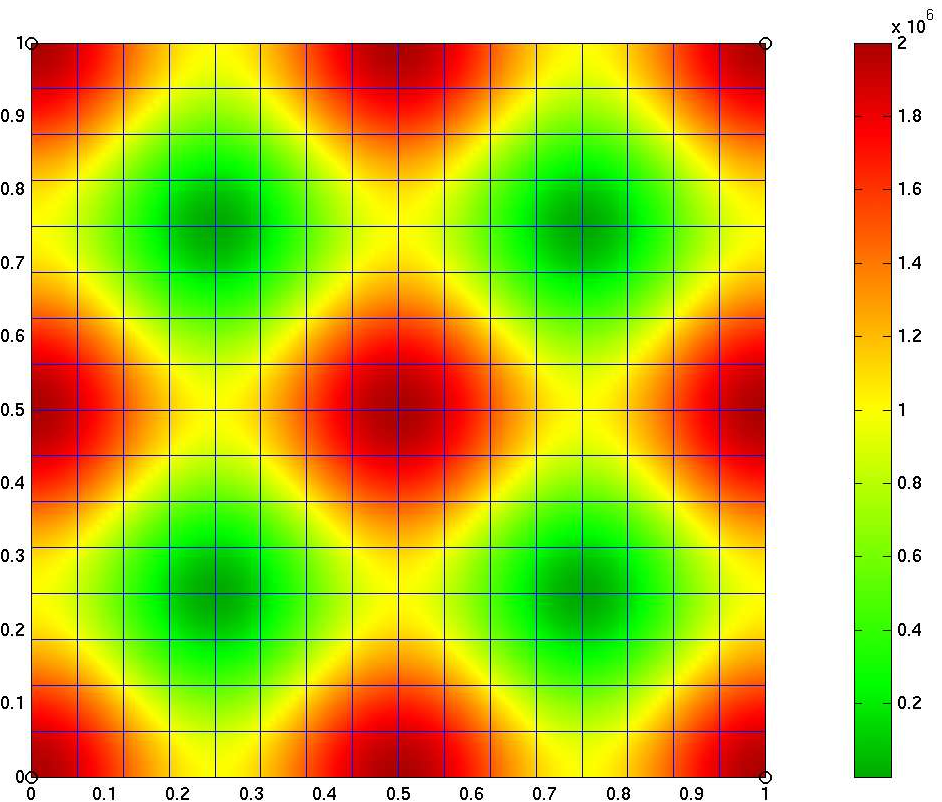
\includegraphics[width=0.48\textwidth]{figs/box}
	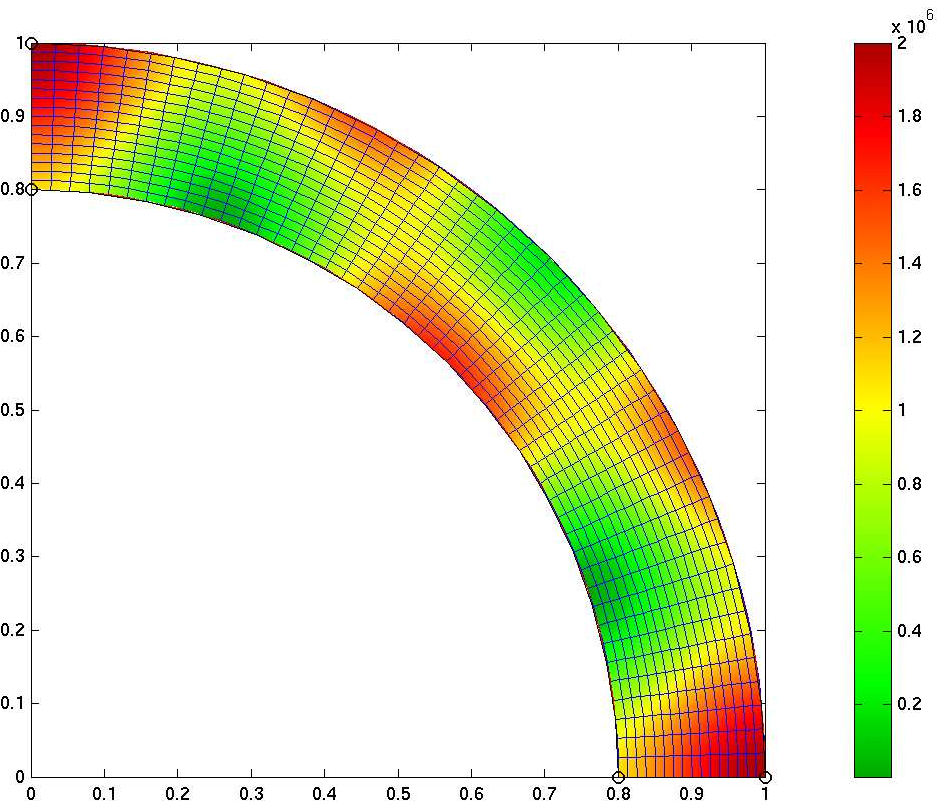
\includegraphics[width=0.48\textwidth]{figs/fan}
	\caption{\label{fig:mesh2d} The two dimensional meshes used in
          our tests. The color corresponds to the value of the
          coefficient $\mu(\bs x)$.}
\end{figure}
\begin{figure}
	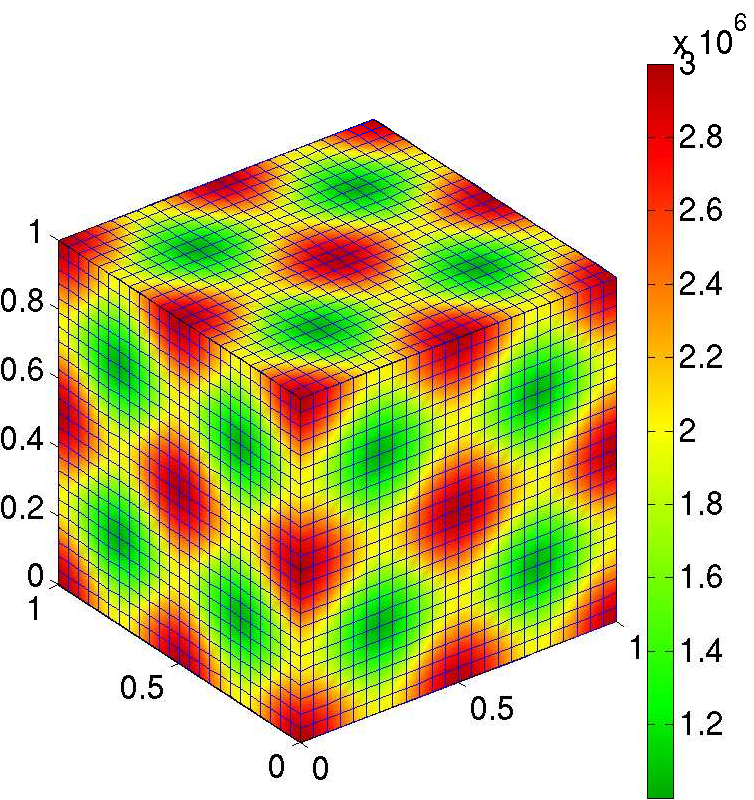
\includegraphics[width=0.48\textwidth]{figs/box3a}
	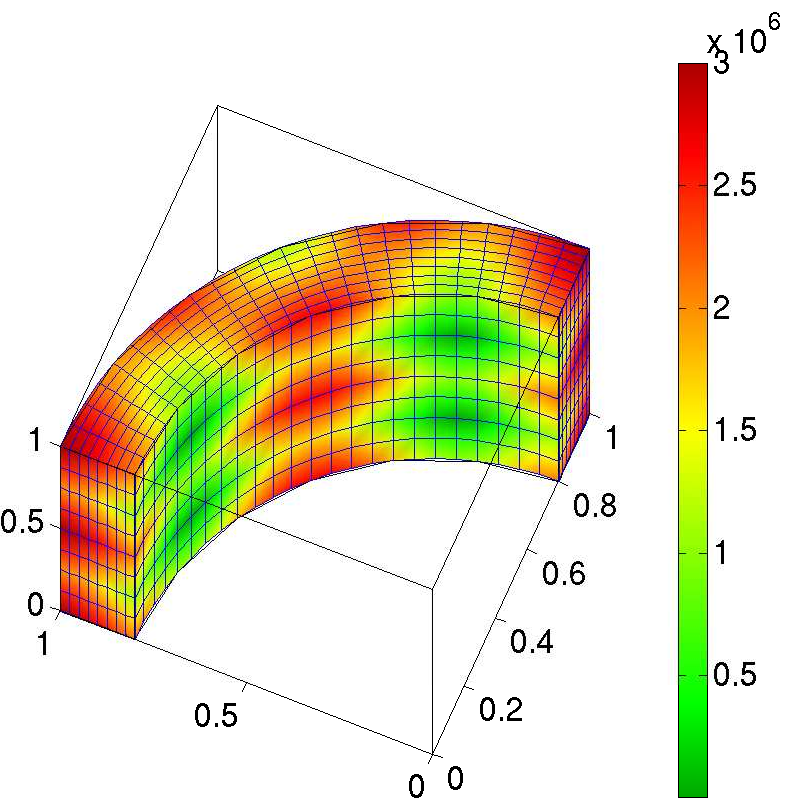
\includegraphics[width=0.48\textwidth]{figs/fan3a}
	\caption{\label{fig:mesh3d} The three dimensional meshes used
          in our tests. The color corresponds to the value of the
          coefficient $\mu(\bs x)$.}
\end{figure}




\subsection{Results for test problems}\label{subsec:results}
Here, we summarize our results for the test problems and present
comprehensive comparisons of the performance of our algorithms for the
solution of high-order discretizations of \eqref{eq:Poisson}.  The
Tables~\ref{tab:box}\ldots present the number of multigrid v-cycles or
of conjugate gradient (CG) iterations required to reduce the norm of
the discrete residual by a factor of $10^8$ for our test problems. In
particular, these tables show:
\begin{itemize}
\item[$\bullet$] The first column gives the polynomial \emph{order}
  used in the finite element discretization.
\item[$\bullet$] The columns entitled by \emph{MG as solver} report
  the number of v-cycles needed when multigrid is used as a
  solver. The subcolums are:
  \begin{itemize}
  \item \emph{Jacobi(3)} denotes that 3 pre-smoothing and 3
    post-smoothing steps of a pointwise Jacobi smoother are used on
    each level.
  \item \emph{Cheb(3)} denotes that Chebyshev-accelerated Jacobi
    smoothing is used. Again, we use 3 pre-smoothing and 3
    post-smoothing steps. The maximal eigenvalue required by the
    Chebyshev method is estimated using \todo{XX iterations of
      Lanczos}.
  \item \emph{SSOR(2)} denotes that a symmetric successive
    over-relaxation method is employed, where 2 pre-smoothing and 1
    post-smoothing step are employed. Note that each SSOR smoothing
    iteration amounts to a forward and a backward step, and thus
    requires double the computational work compared to Jacobi
    smoothing.\footnote{This ignores aspects occurring in parallel
      environments, where Gauss-Seidel smoothing---such as SSOR---can
      be challenging to implement and requires more communication in
      distributed memory environments.}. The SSOR smoother is based on 
			a lexicographic ordering of  the unknowns. 
			\gsnote{use different ordering too?}
	\end{itemize}
	
  Note that for each of the smoothers we results for high-order
  $h$-multigrid (columns marked by \emph{h}; see
  Section~\ref{subsec:h}) as well as for $p$-multigrid (columns marked
  by \emph{p}; see Section~\ref{subsec:p}). For $p$-multigrid, we
  restrict ourselves to orders that are powers of 2. After coarsening
  in $p$ as till $p=1$, and then coarsen in $h$.
\item[$\bullet$] The columns entitled with \emph{MG with pCG} presents
  our results obtained when multigrid is uses as preconditioner in a
  CG algorithm. The sub-columns are as described above.
\item[$\bullet$] The columns headed by \emph{linearized pCG} present
  the number of CG iterations needed to solve the high-order system
  preconditioned with the low-order operator based on the high-order
  node points (see Section~\ref{subsec:low}). In our implementation,
  the low-order system is solved using a direct factorization method.
  The sub-column headed by \emph{GLL} indicates that the non-evenly
  spaces GLL points are used in the low-order system, where
  \emph{unif.} indicates that a uniform node spacing is used for the
  low-order operator.
\end{itemize}


\begin{table}
  \caption{\label{tab:box} Results for two-dimensional unit square
    with constant coefficient $\mu\equiv 1$.  A total of 3 grids were
    used, the finest grid was $32\times 32$, and the coarsest was
    $8\times 8$ \todo{New}.}
  \centering
  \begin{tabular}{|r|c c|c c|c c||c c|c c|c c||c c|} 
    \hline
    & \multicolumn{6}{c||}{MG as solver} & \multicolumn{6}{c||}{MG with pCG} & \multicolumn{2}{r|}{linearized} \\
    \cline{2-13}
    \!\!\! order \!\!\!\! &  \multicolumn{2}{c|}{\!\scriptsize  Jacobi(3)\!} &  \multicolumn{2}{c|}{\!\scriptsize Cheb(3)\!} & \multicolumn{2}{c||}{\!\scriptsize  SSOR(2)\!} & \multicolumn{2}{c|}{\!\scriptsize Jacobi(3)\!} &  \multicolumn{2}{c|}{\!\scriptsize Cheb(3)\!} & \multicolumn{2}{c||}{\!\scriptsize SSOR(2)\!} & \multicolumn{2}{r|}{pCG}\\
\hline
 & $h$ & $p$ & $h$ & $p$& $h$ & $p$& $h$ & $p$& $h$ & $p$& $h$ & $p$& GLL & unif.\\
 \cline{2-15}
1 & 6 & & 5 & & 5 & & 5 & & 4 & & 4 & & 1 & 1  \\
2 & 7 & 7 & 5 & 5 & 5 & 5 & 6 & 6 & 4 & 4 & 4 & 4 & 16 & 16 \\
3 & 8 & & 6 & & 5 & & 6 & & 5 & & 5 & & 18 & 19  \\
4 & 9 & 8 & 6 & 6 & 5 & 5 & 6 & 6 & 5 & 5 & 5 & 5 & 20 & 22 \\
5 & 12 & & 8 & & 7 & & 7 & & 6 & & 5 & & 22 & 26  \\
6 & 12 & & 9 & & 7 & & 8 & & 6 & & 5 & & 25 & 31  \\
7 & 16 & & 12 & & 8 & & 9 & & 7 & & 6 & & 26 & 36  \\
8 & 17 & 14 & 13 & 10 & 8 & 7 & 9 & 9 & 8 & 7 & 6 & 6 & 28 & 42 \\
16 & 40 & 49 & 33 & 27 & 13 & 11 & 16 & 17 & 13 & 13 & 8 & 8 & 41 & 88\\
\hline
  \end{tabular}
\end{table}


\begin{table}
  \caption{\label{tab:2d-fan} Results for two-dimensional warped geometry
    with varying coefficient \todo{$\mu(\bs x) =$}.}
  \centering
  \begin{tabular}{|r|c c|c c|c c||c c|c c|c c||c c|} 
    \hline
    & \multicolumn{6}{c||}{MG as solver} & \multicolumn{6}{c||}{MG with pCG} & \multicolumn{2}{r|}{linearized} \\
    \cline{2-13}
    \!\!\! order \!\!\!\! &  \multicolumn{2}{c|}{\!\scriptsize  Jacobi(3)\!} &  \multicolumn{2}{c|}{\!\scriptsize Cheb(3)\!} & \multicolumn{2}{c||}{\!\scriptsize  SSOR(2)\!} & \multicolumn{2}{c|}{\!\scriptsize Jacobi(3)\!} &  \multicolumn{2}{c|}{\!\scriptsize Cheb(3)\!} & \multicolumn{2}{c||}{\!\scriptsize SSOR(2)\!} & \multicolumn{2}{r|}{pCG}\\
\hline
 & $h$ & $p$ & $h$ & $p$& $h$ & $p$& $h$ & $p$& $h$ & $p$& $h$ & $p$& GLL & unif.\\
 \cline{2-15}
1 & 5 & & 4 & & 4 & & 5 & & 4 & & 3 & & 1 & 1  \\
2 & 8 & 8 & 5 & 5 & 4 & 5 & 6 & 6 & 4 & 5 & 4 & 4 & 26 & 26 \\
3 & 9 & & 7 & & 5 & & 7 & & 5 & & 5 & & 29 & 33  \\
4 & 11 & 10 & 8 & 7 & 6 & 5 & 7 & 7 & 6 & 5 & 5 & 4 & 33 & 42 \\
8 & 106 & 350 & 46 & 350 & 17 & 15 & 23 & 24 & 20 & 20 & 10 & 10 & 26 & 41 \\
16 & 350 & 350 & 350 & 350 & 35 & 31 & 35 & 37 & 31 & 30 & 14 & 15 & 33 & 72 \\
\hline
  \end{tabular}
\end{table}


\begin{table}
  \caption{\label{tab:3d-box} Results for three-dimensional cube geometry
    with constant coefficient $\mu(\bs x) \equiv 1$.}
  \centering
  \begin{tabular}{|r|c c|c c|c c||c c|c c|c c||c c|} 
    \hline
    & \multicolumn{6}{c||}{MG as solver} & \multicolumn{6}{c||}{MG with pCG} & \multicolumn{2}{r|}{linearized} \\
    \cline{2-13}
    \!\!\! order \!\!\!\! &  \multicolumn{2}{c|}{\!\scriptsize  Jacobi(3)\!} &  \multicolumn{2}{c|}{\!\scriptsize Cheb(3)\!} & \multicolumn{2}{c||}{\!\scriptsize  SSOR(2)\!} & \multicolumn{2}{c|}{\!\scriptsize Jacobi(3)\!} &  \multicolumn{2}{c|}{\!\scriptsize Cheb(3)\!} & \multicolumn{2}{c||}{\!\scriptsize SSOR(2)\!} & \multicolumn{2}{r|}{pCG}\\
\hline
 & $h$ & $p$ & $h$ & $p$& $h$ & $p$& $h$ & $p$& $h$ & $p$& $h$ & $p$& GLL & unif.\\
 \cline{2-15}
1 & 5 & & 4 & & 4 & & 5 & & 4 & & 3 & & 1 & 1  \\
2 & 8 & 8 & 5 & 5 & 4 & 5 & 6 & 6 & 4 & 5 & 4 & 4 & 26 & 26 \\
3 & 9 & & 7 & & 5 & & 7 & & 5 & & 5 & & 29 & 33  \\
4 & 11 & 10 & 8 & 7 & 6 & 5 & 7 & 7 & 6 & 5 & 5 & 4 & 33 & 42 \\
\hline
5 & 14 & & 10 & & 5 & & 8 & & 7 & & 5 & & 36 & 50  \\
6 & 16 & & 12 & & 6 & & 9 & & 8 & & 5 & & 40 & 61  \\
7 & 20 & & 15 & & 7 & & 10 & & 9 & & 5 & & 44 & 74  \\
8 & 22 & 18 & 17 & 15 & 7 & 6 & 11 & 10 & 10 & 8 & 5 & 5 & 52 & 99 \\
\hline
  \end{tabular}
\end{table}

\begin{table}
  \caption{\label{tab:3d-fan} Results for three-dimensional warped geometry
    with varying coefficient \todo{$\mu(\bs x)=$}.}
  \centering
  \begin{tabular}{|r|c c|c c|c c||c c|c c|c c||c c|} 
    \hline
    & \multicolumn{6}{c||}{MG as solver} & \multicolumn{6}{c||}{MG with pCG} & \multicolumn{2}{r|}{linearized} \\
    \cline{2-13}
    \!\!\! order \!\!\!\! &  \multicolumn{2}{c|}{\!\scriptsize  Jacobi(3)\!} &  \multicolumn{2}{c|}{\!\scriptsize Cheb(3)\!} & \multicolumn{2}{c||}{\!\scriptsize  SSOR(2)\!} & \multicolumn{2}{c|}{\!\scriptsize Jacobi(3)\!} &  \multicolumn{2}{c|}{\!\scriptsize Cheb(3)\!} & \multicolumn{2}{c||}{\!\scriptsize SSOR(2)\!} & \multicolumn{2}{r|}{pCG}\\
\hline
 & $h$ & $p$ & $h$ & $p$& $h$ & $p$& $h$ & $p$& $h$ & $p$& $h$ & $p$& GLL & unif.\\
 \cline{2-15}
1 & 350 & & 10 & & 4 & & 11 & & 7 & & 4 & & 1 & 1  \\
2 & 20 & 21 & 18 & 18 & 7 & 7 & 10 & 10 & 9 & 10 & 5 & 5 & 27 & 27 \\
3 & 25 & & 21 & & 8 & & 11 & & 10 & & 6 & & 30 & 33  \\
4 & 29 & 27 & 24 & 23 & 9 & 9 & 12 & 12 & 11 & 11 & 6 & 6 & 32 & 42 \\
5 & 36 & & 30 & & 11 & & 14 & & 13 & & 7 & & 35 & 50  \\
6 & 41 & & 34 & & 13 & & 15 & & 14 & & 8 & & 38 & 60  \\
7 & 48 & & 40 & & 14 & & 17 & & 15 & & 8 & & 40 & 70  \\
8 & 50 & 45 & 42 & 38 & 15 & 14 & 17 & 16 & 16 & 14 & 9 & 8 & 40 & 81 \\
\hline
  \end{tabular}
\end{table}


\section{Discussion and conclusions}

%Finalize and discuss ramifications.

\todo{Preliminary list of conclusions:}
\begin{itemize}
\item Chebyshev improves significantly over Jacobi smoothing and is
  competitive with SSOR
\item Point smoothers performed reasonably well for all tested orders,
  in particular in combination with pCG
\item low-order preconditioner competitive w.r. to number of
  iterations; thus a good option as preconditioner when using AMG for
  unstructured high-order meshes

%\item Using Jacobi-based multigrid as preconditioner in the conjugate
%  gradient method, the number of iterations for polynomial orders
%  $p=2,3$ is similar to the number of iterations for linear elements.
%  In general, for the same number of unknowns one can expect better
%  accuracy for higher polynomial order. This advantage has to be
%  contrasted with the fact that high-order operators are less sparse
%  and thus their application to vectors is more time consuming.  Using
%  Jacobi-based smoothers is attractive from a parallel perspective
%  since no coloring of unknowns as in SSOR is necessary.
%\item Both, high-order $h$-multigrid as well as $p$-multigrid yield
%  significantly faster convergence in terms of the number of
%  iterations than preconditioning with the low-order
%  operator. Although low order operators are sparser and thus faster
%  to apply, the significant larger number of iterations results in
%  larger time-to-solution, in particular since the high-order operator
%  must be used to compute the residual on the finest mesh.
%\item For problems that only require a small number of smoothing
%  steps, using Chebyshev acceleration for the Jacobi smoother does not
%  improve the convergence. In all our tests, SSOR smoothing results in
%  the fastest convergence, in particular for orders $p\ge
%  4$. \gsnote{Revisit.}
\end{itemize}


\bibliographystyle{siam}
\bibliography{ccgo}


\end{document}
